\chapter{Exploratory Data Analysis}

\epigraph{Cricket often leaves you scratching your head}{James Anderson}

The purpose of this chapter is to explore the obtained dataset in more detail. This is necessary for carrying out the work in later chapters. In general, and no less
in the world of statistics, making assumptions is dangerous, and so in order to make the assumptions we do in later chapters, we must have the evidence to back it up.
This chapter not only provides that evidence, but allows us to become more familiar with our dataset, and see how modern data fits in with the previous work done in this 
field. \\
We begin by looking at the probability densities in the Fall of Wicket variables. F.o.W is key in the DLS method, so we do this to get an idea of what lies underneath the
surface. We are able to explain the way F.o.W distributions are shaped based onthe way cricket games unfold. This consistency allows us to make an assumption about Runrates
later in the chapter too. 
As with any dataset, there are outliers, and the number of such will have influence on the error function that we use in later models. For that reason, we give brief discussion 
to this, before going on to look at whether or not scores in games of cricket are normally distributed around some mean. \\
Runrates are the discussed in more detail, looking at whether or not the runrates in certain periods of the game also follow a normal distribution. Finding this out is imperative
for using Monte-Carlo simmulation later on in the paper.

\section{Fall of Wicket Densities}

In this chapter, we are looking only at the first innings of the games, and only those games in which the full 50 overs were played. The 
reason for this is the models we will build are going to try and predict a score as if a full innings has been played. \\

We begin our exploration of the data with a look at how the density of the runs scored per fall of wicket changes. This has been done for each
individual team in the dataset, and in figures \ref{ovrdens1fow}-\ref{ovrdens9fow}, we can see how this evolves.  

\begin{figure}[h]
    \centering
    \begin{minipage}{0.4\textwidth}
        \centering
        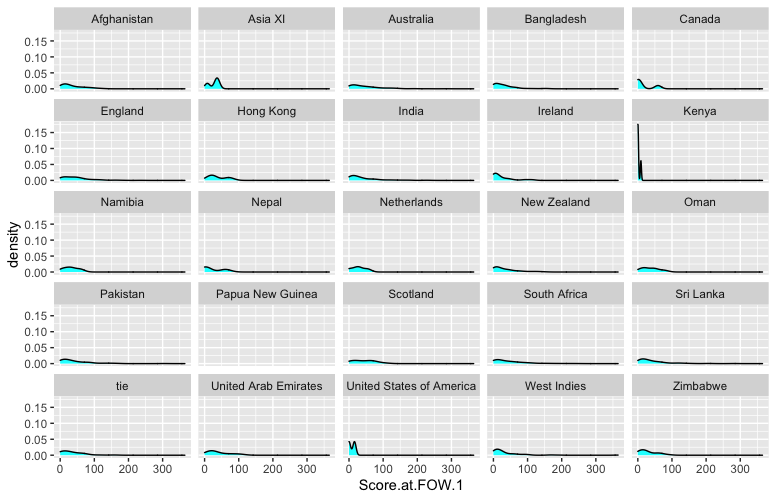
\includegraphics[scale=0.3]{figures/fow1density.png}
        \caption{Density of all teams for first wicket falling}
        \label{alldens1fow}
    \end{minipage}
    \begin{minipage}{0.4\textwidth}
        \centering
        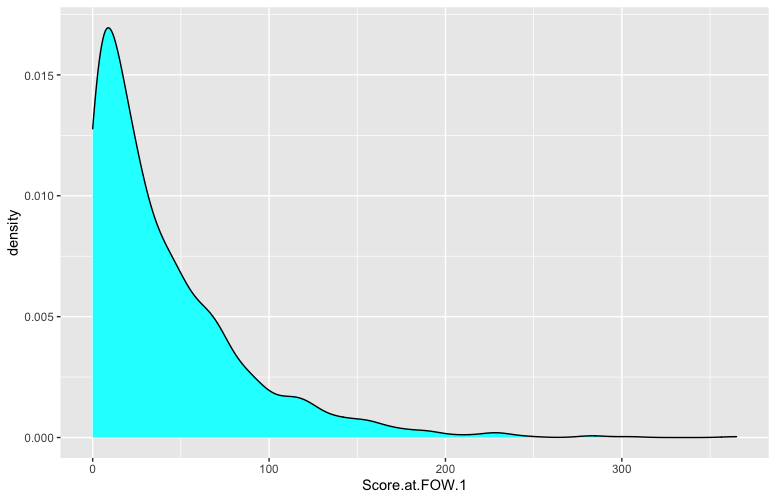
\includegraphics[scale=0.3]{figures/fow1densFull.png}
        \caption{Overall density plot for FOW 1}
        \label{ovrdens1fow}
    \end{minipage}
\end{figure}

\begin{figure}[h]
    \centering
    \begin{minipage}{0.4\textwidth}
        \centering
        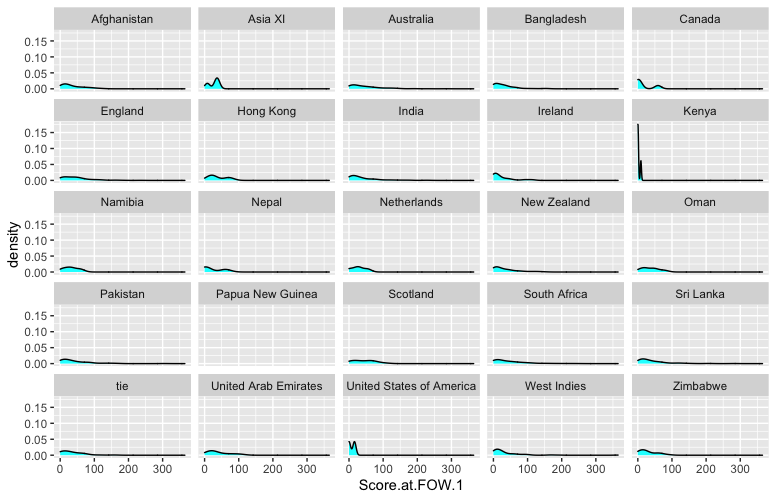
\includegraphics[scale=0.3]{figures/fow1density.png}
        \caption{Density of all teams for fith wicket falling}
        \label{alldens5fow}
    \end{minipage}
    \begin{minipage}{0.4\textwidth}
        \centering
        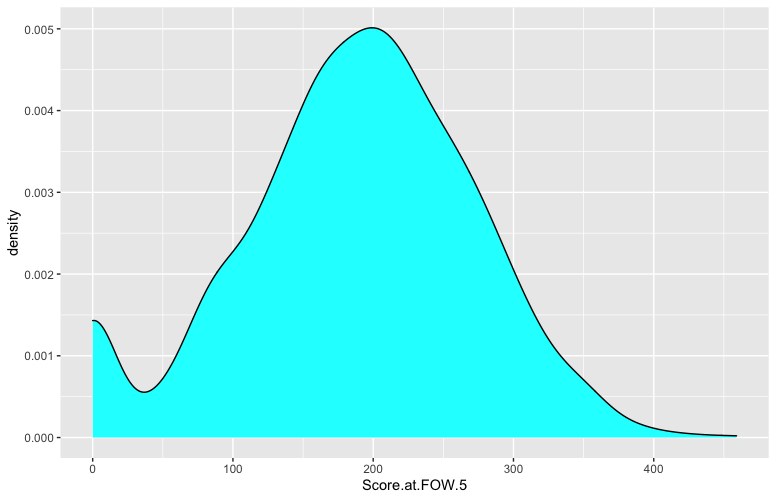
\includegraphics[scale=0.3]{figures/fow5densFull.png}
        \caption{Overall density plot for FOW 5}
        \label{ovrdens5fow}
    \end{minipage}
\end{figure}

\begin{figure}[h]
    \centering
    \begin{minipage}{0.4\textwidth}
        \centering
        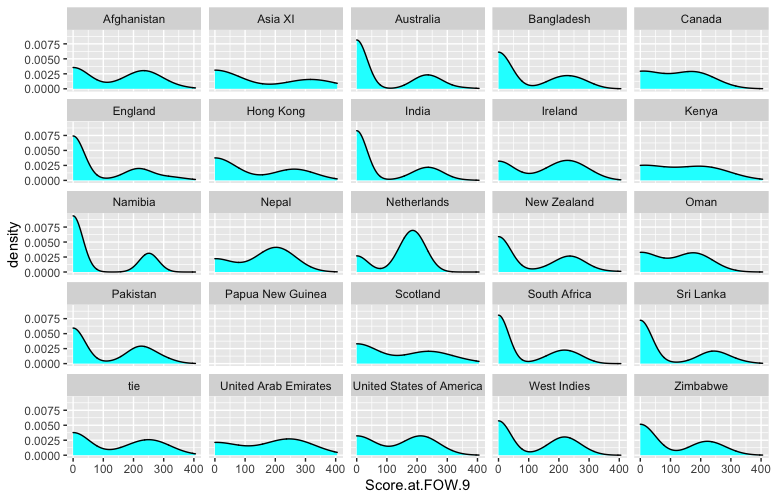
\includegraphics[scale=0.3]{figures/fow9density.png}
        \caption{Density of all teams for ninth wicket falling}
        \label{alldens9fow}
    \end{minipage}
    \begin{minipage}{0.4\textwidth}
        \centering
        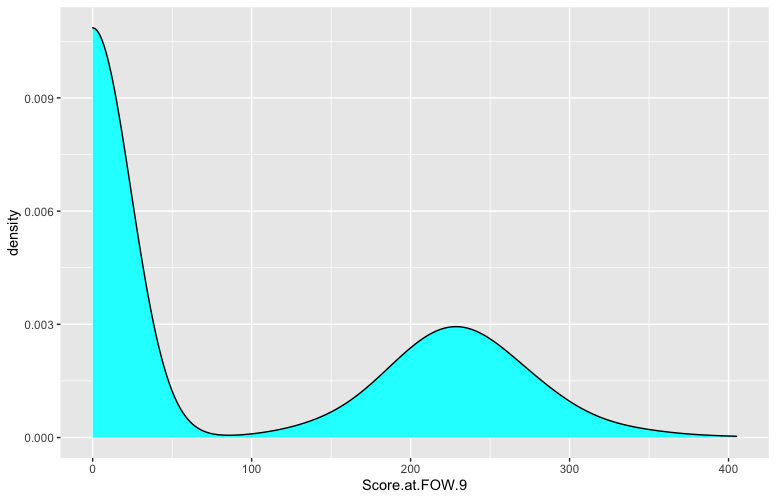
\includegraphics[scale=0.3]{figures/fow9densfull.png}
        \caption{Overall density plot for FOW 9}
        \label{ovrdens9fow}
    \end{minipage}
\end{figure}

In \ref{ovrdens1fow}, we see the density is heavily skewed to the left. This makes sense, as the bowling team will presumably be starting 
their innings by using their best bowlers, who will be hunting to get wickets early on. In \ref{ovrdens5fow}, we see a much more normally distributed
density function. But in actual fact, we see this interesting second, smaller peak appearing lower down in the score. Does this make sense? It's certainly 
not suprising. What these two peaks exemplify is the fact games can go heavily in favour of the bowling team, which can be seen in the first small peak,
wherein they have taken a lot of wickets in quick succession, meaning the later order batters are coming in earlier than usual. Secondly, it shows when the 
batting team is having a good day, because we have this much larger peak around the 200 runs mark.\\

Finally, in \ref{ovrdens9fow}, we can see that the earlier bowling advantage peak is much higer, because the lower order batters are traditionally less skilled 
at batting, and so the bowling team have a distinct advantage in taking wickets against these players. But we also see the second, batting-favoured peak is no much lower.
This corresponds to the scenario in which the earlier batters have laid a good foundation of the game, and the lower-order batters have not had to contribute much to the score.

\section{Outliers in Runs Data}
\label{mse}
In the next chapter, it will be necessary to choose a loss function for improving the neural network that we create. To aid in determining this, we need to look at the
spread of runs scored in a full innings of data. This can be seen in \ref{runsbox}.

\begin{figure}[h]
    \centering
    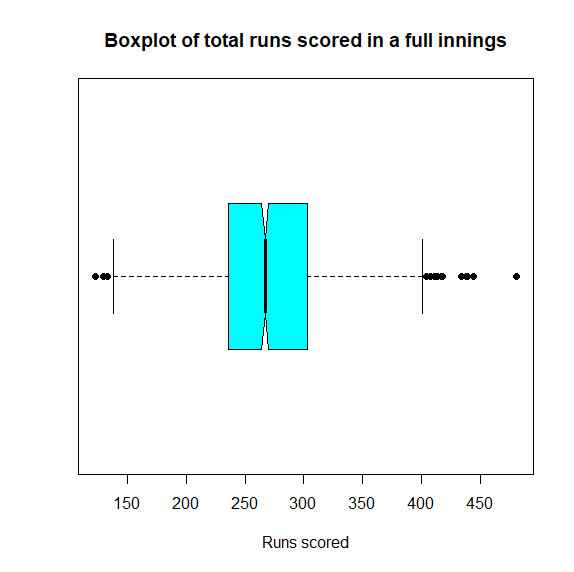
\includegraphics[width=0.4\linewidth]{figures/runsbox.png}
    \caption{Boxplot showing the spread of runs scored}
    \label{runsbox}
\end{figure}

There are 363 data points greater than the third quartile, while 671 are below the first quartile. So $25.3\%$ of our data lies above the third quartile, and
$46.7\%$ below the first. For that reason, we make the decision to use the Mean-Squared-Error (MSE) loss function, which is commonplace in regression problems.

\section{On the Normality of Run Totals}
It will be useful in later parts of this dissertation to know whether or not scores are normally distributed. To test whether or not 
they are, we use a Q-Q plot to check. This is a graphical way for checking normality, by comparing the quantiles of a dataset (in this case, scores) to quantiles
drawn from a theoretical distribution. If the resulting points follow a straight line, it is likely that the data came from the distribution.
In this case, we use the R function \textit{qqnorm()} to test if the runs from the 1436 games of a full 50 overs follow a normal distribution.

\begin{figure}[h]
    \label{qqplot}
    \centering
    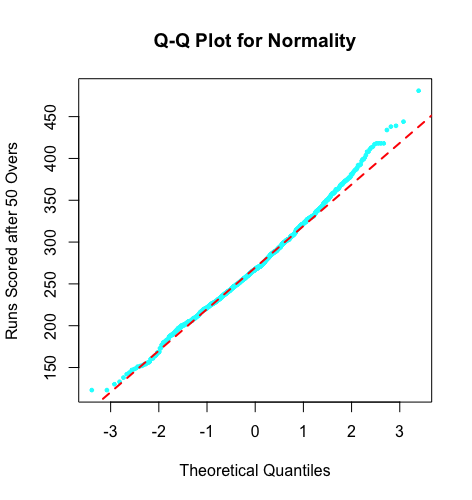
\includegraphics[width=0.4\linewidth]{figures/qqnormplot.png}
    \caption{Q-Q plot for runs scored after 50 overs.}
\end{figure}

We can see from the above figure that the plot follows along the straight line and so we can conclude that the scores are infact normally distributed. 
Further, we can calculate the parameters of this distribution using the R functions \textit{mean()} and \textit{var()}. Doing so gives that the distribution
of scores in 50 overs, $S_{50}$, can be given as $S_{50} \sim \mathcal{N}(270.56,51.34^2)$. \\ 

To further test that this is indeed the case, we can create a sample plot based on this distribution, which can be seen in figure \ref{samplenorm}

\begin{figure}[h]
    \label{samplenorm}
    \centering
    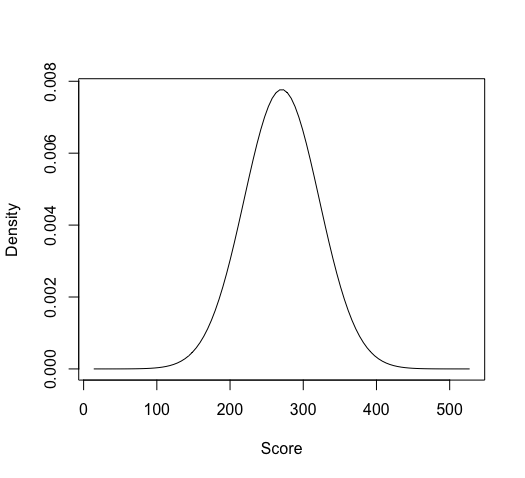
\includegraphics[width=0.4\linewidth]{figures/samplenorm.png}
    \caption{Sample plot created from the derived distribution of $S_{50}$}
\end{figure}

With this in mind, we can now look at a density plot for the actual data. This is giving in figure \ref{runsdens}.

\begin{figure}[h]
    \centering
    \subfloat[\centering Density for Runs Scored]{{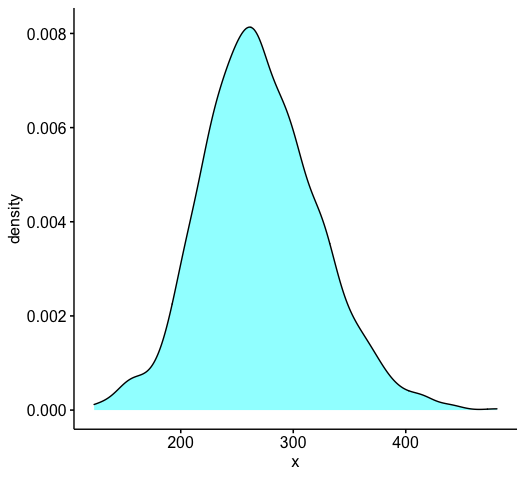
\includegraphics[width=.4\linewidth]{figures/runsdensity.png} }}
    \qquad
    \subfloat[\centering Q-Q Plot for First Innings]{{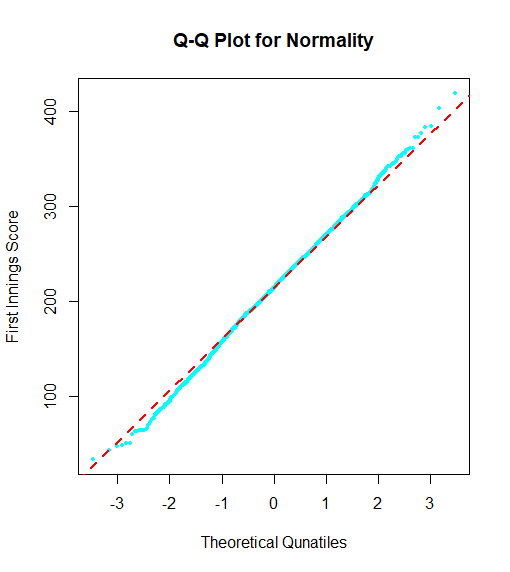
\includegraphics[width=.4\linewidth]{figures/firstInnsQQ.png} }}
    \label{errDistAndQQ}
\end{figure}

It is unsuprising that runs are normally distributed, but to be able to draw a mean and variance from this will be very helpful in future aspects of the project.

We have seen that first innings scores in a full 50 overs are normally distributed. We can check, using the same methods if runs in a first innings that 
doesn't necessarily go for the full allowance of overs is normally distributed. 

We find that $S_{FI} \sim \mathcal{N}(213.49,56.91^2)$. 

\section{Runrates}
\label{exprr}
The work that follows in this section is essential to allowing the Neural Network constructed in Chapter 5 to predict the scores of games. The aim of this section is 
to see if we can draw the runrates at specific overs from a statistical distribution. This will in turn enable us to fill the gaps in the missing overs of a game. In turn, 
with the gaps filled, we can pass the simmulated runrates to the neural network, and allow for a score to be predicted. 

\begin{figure}[h]
    \centering
    \subfloat[\centering Average runnrate per over]{{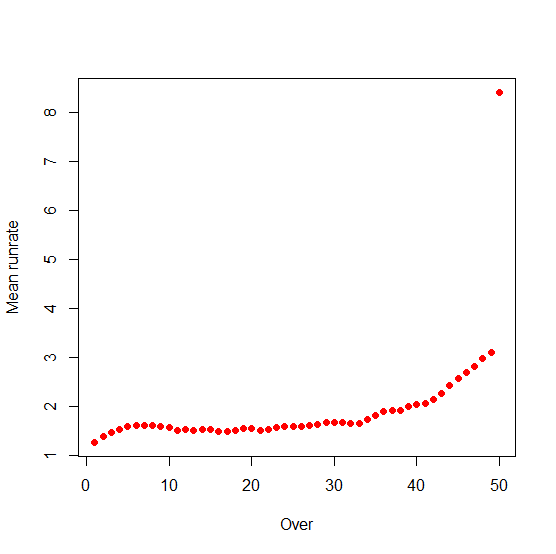
\includegraphics[width=.4\linewidth]{figures/avgRR.png} }}
    \qquad
    \subfloat[\centering Runrate Standard deviation per over]{{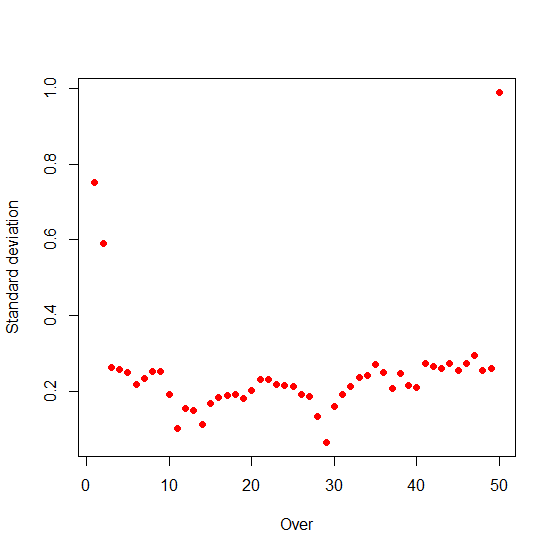
\includegraphics[width=.4\linewidth]{figures/sdrr.png} }}
    \caption{Error distribution with Q-Q plot}
    \label{errdistqq3}
\end{figure}

We can see from this figure, that average runrate seems to stay consistent in the middle overs, before rapidly increasing as the risk associated with losing 
a wicket falls off due to the end of the innings coming closer. If we break the game into five ten-over segments, as these are generally different periods of the game
from a tactical perspective\footnote{This is to do with different bowling options being used to be more effective as the pitch conditions change}, we can model the segments.
A game of ODI-cricket can roughly be broken up to three segments, the first 10 overs, known as the ``powerplay'', where teams are slightly more conservative and look to build a 
foundation on which the rest of the game is built. The middle overs are 11-35. The idea of this game is to continue building on the foundation, and save wickets. The last 
15 overs are where more risks are taken, as the value of a wicket decreases. The mentality is to double your score from the first 35 in the last 15, that is why we see the massive 
increase in runrate in these last overs. \\

Using this information, we can create density plots of the average runrate in these overs, as in figures 4.13-4.15. 

\begin{figure}[h]
    \minipage{0.32\textwidth}
      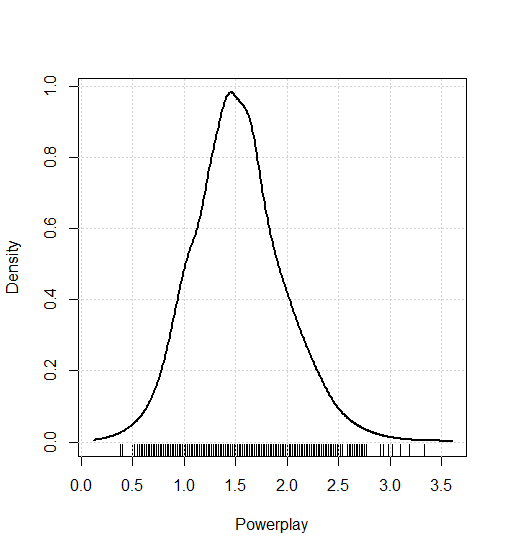
\includegraphics[width=\linewidth]{figures/powerplaydens.png}
      \caption{Powerplay runrate density}
    \endminipage\hfill
    \minipage{0.32\textwidth}
      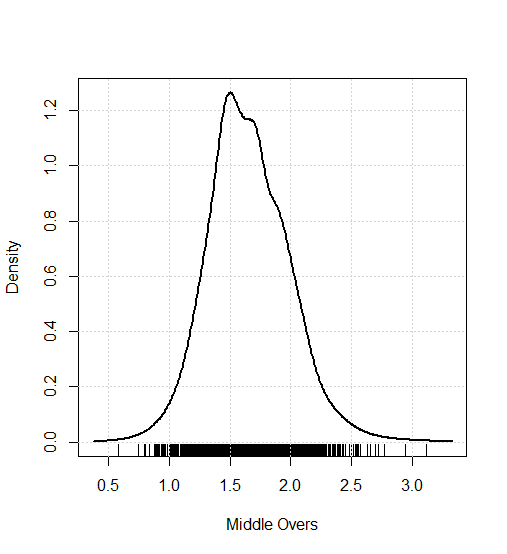
\includegraphics[width=\linewidth]{figures/middleoversdens.png}
      \caption{Middle Overs runrate density}
    \endminipage\hfill
    \minipage{0.32\textwidth}%
      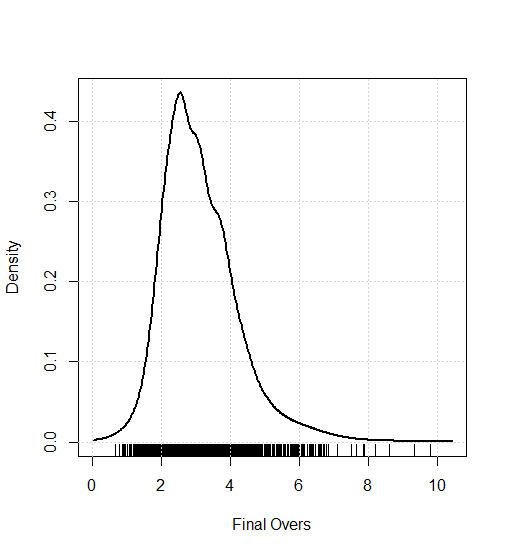
\includegraphics[width=\linewidth]{figures/finaloversdens.png}
      \caption{Final Overs density}
    \endminipage
\end{figure}

The runrates are roughly normally distributed. It is reasonable that due to the Central Limit Theorem, with more observations, these distribiutions would be smoothed out and 
appear more normally distributed than it does at present. This is imporant, because it allows us to use our 